% ****** Start of file apssamp.tex ******
%
%   This file is part of the APS files in the REVTeX 4.1 distribution.
%   Version 4.1r of REVTeX, August 2010
%
%   Copyright (c) 2009, 2010 The American Physical Society.
%
%   See the REVTeX 4 README file for restrictions and more information.
%
% TeX'ing this file requires that you have AMS-LaTeX 2.0 installed
% as well as the rest of the prerequisites for REVTeX 4.1
%
% See the REVTeX 4 README file
% It also requires running BibTeX. The commands are as follows:
%
%  1)  latex apssamp.tex
%  2)  bibtex apssamp
%  3)  latex apssamp.tex
%  4)  latex apssamp.tex
%
\documentclass[%
%reprint,
%superscriptaddress,
%groupedaddress,
%unsortedaddress,
%runinaddress,
%frontmatterverbose, 
preprint,
%showpacs,preprintnumbers,
%nofootinbib,
%nobibnotes,
%bibnotes,
 amsmath,amssymb,
 aps,
%pra,
%prb,
%rmp,
%prstab,
%prstper,
%floatfix,
]{revtex4-1}

\usepackage{graphicx}% Include figure files
\usepackage{dcolumn}% Align table columns on decimal point
\usepackage{bm}% bold math
%\usepackage{hyperref}% add hypertext capabilities
%\usepackage[mathlines]{lineno}% Enable numbering of text and display math
%\linenumbers\relax % Commence numbering lines

%\usepackage[showframe,%Uncomment any one of the following lines to test 
%%scale=0.7, marginratio={1:1, 2:3}, ignoreall,% default settings
%%text={7in,10in},centering,
%%margin=1.5in,
%%total={6.5in,8.75in}, top=1.2in, left=0.9in, includefoot,
%%height=10in,a5paper,hmargin={3cm,0.8in},
%]{geometry}


%%%%%%%%%%%%%%%%%%%%%%%%%%%
%%%%%%  PREAMBLES %%%%%%%%%
\newcommand{\ud}[1]{{#1^{\dagger}}}
\newcommand{\bra}[1]{\left\langle #1\right|}
\newcommand{\ket}[1]{\left| #1\right\rangle}
\newcommand\Tr{\mathrm{Tr}}
\newcommand{\braket}[2]{\langle #1 \mid #2 \rangle}
\newcommand\I{\mathbb{I}}
\newcommand{\avg}[1]{\left< #1 \right>}
\newcommand{\sech}[1]{{\operatorname{sech}{#1}}}
\newcommand{\csch}[1]{{\operatorname{csch}{#1}}}
%%%%%%  PREAMBLES %%%%%%%%%
%%%%%%%%%%%%%%%%%%%%%%%%%%%

\begin{document}

%\preprint{APS/123-QED}

\title{Stimulated Neutrino Oscillations - A Rabi Oscillation View}% Force line breaks with \\
%\thanks{A footnote to the article title}%

\author{Lei Ma}
\email{leima@unm.edu}
\author{Shashank Shalgar}%
\email{shashankshalgar@unm.edu}
\author{Huaiyu Duan}%
\email{duan@unm.edu}
\affiliation{%
 Department of Physics \& Astronomy, University of New Mexico,
 Albuquerque, NM 87131, USA
}%
% \author{Huaiyu Duan}%
%  \email{Second.Author@institution.edu}
% \affiliation{%
%  Authors' institution and/or address\\
%  This line break forced with \textbackslash\textbackslash
% }%

% \collaboration{MUSO Collaboration}%\noaffiliation

% \author{Shashank Shalgar}
%  \homepage{http://www.Second.institution.edu/~Charlie.Author}
% \affiliation{
%  Second institution and/or address\\
%  This line break forced% with \\
% }%
% \affiliation{
%  Third institution, the second for Charlie Author
% }%
% \author{Delta Author}
% \affiliation{%
%  Authors' institution and/or address\\
%  This line break forced with \textbackslash\textbackslash
% }%

% \collaboration{CLEO Collaboration}%\noaffiliation

% \author{Huaiyu Duan}
%  \homepage{http://www.Second.institution.edu/~Charlie.Author}
% \affiliation{
%  Second institution and/or address\\
%  This line break forced% with \\
% }%
% \affiliation{
%  Third institution, the second for Charlie Author
% }%
% \author{Delta Author}
% \affiliation{%
%  Authors' institution and/or address\\
%  This line break forced with \textbackslash\textbackslash
% }%

% \collaboration{CLEO Collaboration}%\noaffiliation



\date{\today}% It is always \today, today,
             %  but any date may be explicitly specified

\begin{abstract}
ABSTRACT PLACEHOLDER
% \begin{description}
% \item[Usage]
% Secondary publications and information retrieval purposes.
% \item[PACS numbers]
% May be entered using the \verb+\pacs{#1}+ command.
% \item[Structure]
% You may use the \texttt{description} environment to structure your abstract;
% use the optional argument of the \verb+\item+ command to give the category of each item. 
% \end{description}
\end{abstract}

% \pacs{Valid PACS appear here}% PACS, the Physics and Astronomy
                             % Classification Scheme.
%\keywords{Suggested keywords}%Use showkeys class option if keyword
                              %display desired
\maketitle

%\tableofcontents

\section{\label{introduction}Introduction}

\begin{enumerate}
    \item Work done before, but the physics is not clear
    \item Decompose the system into Rabi oscillations
\end{enumerate}


\section{\label{rabi}Neutrino Oscillations and Rabi Oscillation}


%% 

\begin{itemize}
    \item Neutrino oscillations in matter (background matter basis)
    \item Rabi oscillations
    \item Width, detuning, and Rabi frequency, and their significance. (Relation to amplitude and oscillation wavelength)
    \item Interference: destruction
\end{itemize}


\subsection{Neutrino oscillations in matter}


\begin{itemize}
    \item The formalism
    \item What has been found before
\end{itemize}


Matter profile

\begin{equation}
    \lambda(x) = \lambda_0 + \delta \lambda (x),
\end{equation}

where

\begin{align}
    \lambda_0 &= \sqrt{2}G_F n_{e0}. \\
    \delta \lambda (x) &= \sqrt{2}G_F \delta n_{e}(x)
\end{align}

We use

\begin{equation}
\delta \lambda = A \sin (k x).
\end{equation}


\fbox{Question: Should we use $A\cos(kx)$ to make comparision with Rabi oscillation?}


Choose $\lambda_0 = 0.5\lambda_{\mathrm{MSW}}$. (For easier reading, specify the actual number density for some characteristic energy such as 10\;MeV.)


In background basis, Hamiltonian becomes

\begin{equation}
    H^{(m)} = - \frac{\omega_m}{2} \sigma_3 + \frac{1}{2}A \sin (k x) \cos 2\theta_m \sigma_3 - \frac{1}{2}A\sin(kx) \sin 2 \theta_m \sigma_1.
\end{equation}


At resonance, $k=\omega_m$, the $\sigma_3$ component of perturbation has no effect when the system is at resonance, as we would prove later more rigorously.






%%%%%%%%%
%%%%%%%%% Rabi oscillation
%%%%%%%%%

\subsection{Rabi oscillation}

\begin{equation}
H_{\mathrm R} = -\frac{\omega_m}{2} \sigma_3 - \frac{1}{2}A_1 \cos(k_1 x) \sigma_1 + \frac{1}{2} A_1 \sin(k_1 x) \sigma_2,
\end{equation}

which is equivalent to

\begin{equation}
H_{\mathrm R} = -\frac{\omega_m}{2} \sigma_3 - \frac{A_1}{2} \begin{pmatrix}0 & e^{i k_1 x} \\ e^{-i k_1 x} & 0 \end{pmatrix} 
\end{equation}


Probability

\begin{equation}
P(x) = \frac{\lvert A_1 \rvert^2}{ \Omega_R^2 }  \sin^2 \left( \Omega_R x/2 \right).
\end{equation}

Rabi frequency

\begin{equation}
\Omega_{\mathrm R} = \sqrt{ \lvert A_1 \rvert^2 + (k_1 - \omega_m)^2 },
\end{equation}

$k_1 - \omega_m$ is the detuning.




\begin{enumerate}
    \item Significance of $A_1$, detuning $k_1 - \omega_m$, and Rabi frequency $\Omega_{\mathrm R}$.
        \begin{itemize}
            \item $\lvert A_1 \rvert$ is the width of the resonance.
            \item $Q = \lvert k_1 - \omega_m \rvert/\lvert A_1 \rvert$ (relative detuning?) determines how close to exact resonance.
            \item $\Omega_{\mathrm R}$ determines the oscillation wavelength. The order of the wavelength is determined by the width, as long as the system is not too far away from exact resonance.
        \end{itemize}
    \item Interference: destruction
        \begin{itemize}
            \item First mode is on exact resonance,  $k_1 = \omega_m$.
            \item Add in a new perturbation with $k_2\ll k_1$, so that
            
            \begin{equation}
            H_{\mathrm R}' = -\frac{\omega_m}{2} \sigma_3 - \frac{1}{2}( A_1 \cos(k_1 x) + A_2 \cos(k_2 x)) \sigma_1 + \frac{1}{2} ( A_1 \sin(k_1 x) + A_2 \sin(k_2 x)   ) \sigma_2.
            \end{equation}
            
            \item The slow mode will change the energy gap, $\omega_m' = \sqrt{\omega_m^2 + A_2^2} \approx \omega_m + \frac{A_2^2}{2\omega_m}$, to significantly decrease the amplitude we need a large $A_2$ which satisfies $\lvert \omega_m' - k_1 \rvert \gg A_1$.
            \item A plot showing that this approximation actually works.
        \end{itemize}
\end{enumerate}


Design a Rabi oscillation system with one mode on exact resonance and a slow modes,

\begin{equation}
H_{\mathrm R}' = -\frac{\omega_m}{2} \sigma_3 - \frac{1}{2}( A_1 \cos(k_1 x) + A_2 \cos(k_2 x)) \sigma_1 + \frac{1}{2} ( A_1 \sin(k_1 x) + A_2 \sin(k_2 x)   ) \sigma_2.
\end{equation}

where $k_1 = \omega_m$, and $k_1 \gg k_2$.

The new energy gap can be predicted

\begin{equation}
\omega_m' = \sqrt{\omega_m^2 + A_2^2}
\end{equation}

Predict the critical $A_2$ that significantly reduces the transition amplitude by setting the detuning value larger than the width,

\begin{equation}
\lvert k_1 - \omega_m' \rvert \gtrsim \text{width of resonance}.
\end{equation}




Figure \ref{fig-rabi-oscillations-energy-gap-change} shows that this hypothesis works. {\bf Maybe a plot that shows the comparison of the predicted amplitudes and numerical amplitudes for different $A_2$'s.}


\begin{figure}[!htbp]
                \centering
                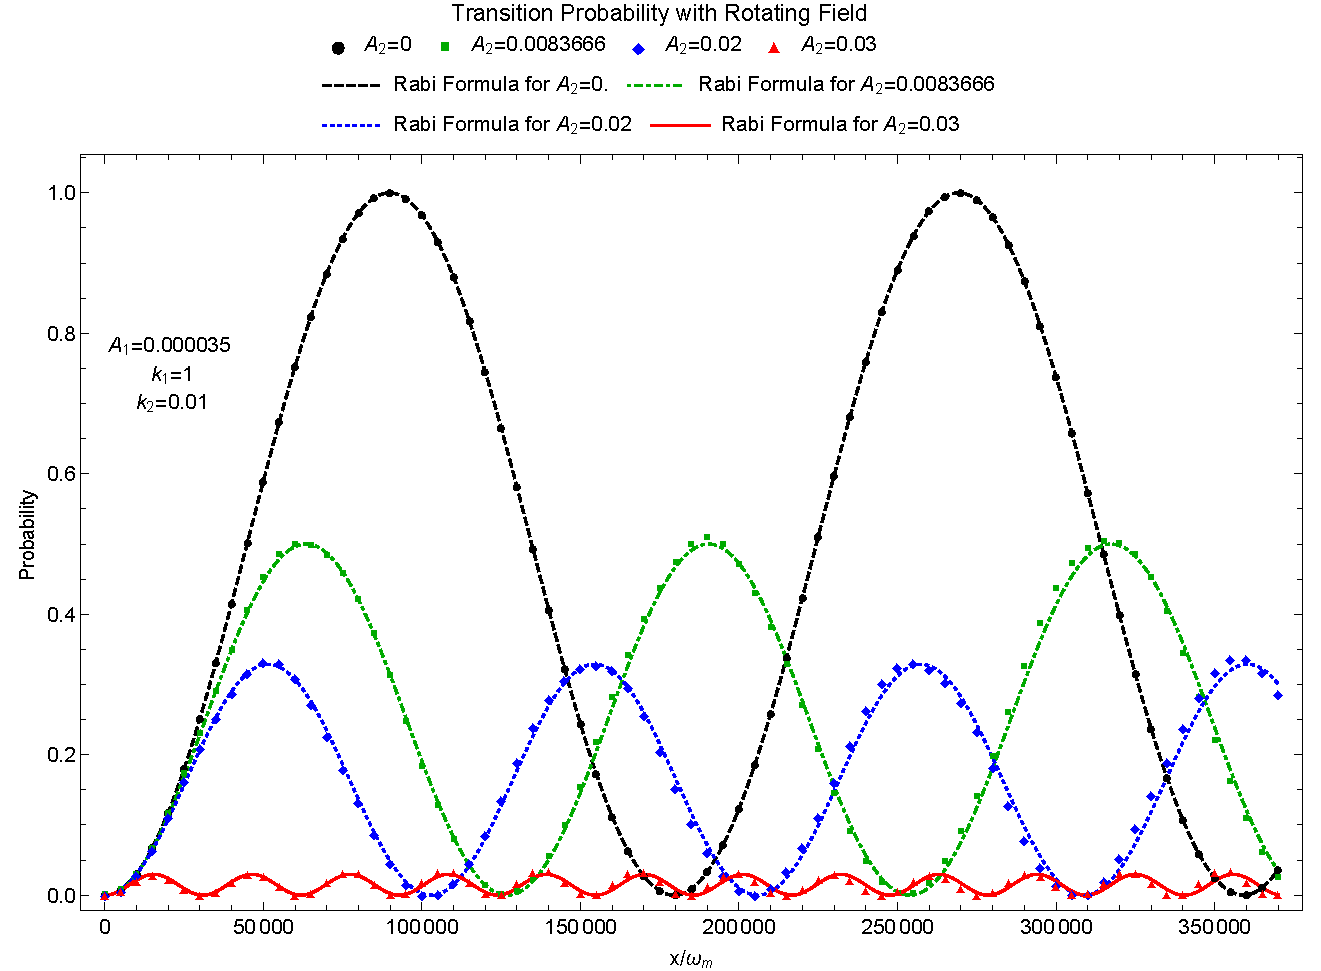
\includegraphics[width=\textwidth]{assets/rabi-oscillations-energy-gap-change-k2-0-01}
                \caption{Reduction of transition amplitudes. Black dashed line: the system has only one perturbation which is at exact resonance; Green dash-dotted line: $A_2=A_{2,\mathrm{Critical}}=0.0083666$; Blue dotted line: $A_2=0.01$; Red line: $A_2=0.02$. The markers are the probabilities predicted using Rabi formula correspondingly. Black cross is the transition probability between two background mass eigenstates for the neutrinos with matter perturbation $A\sin(kx)$.}
                \label{fig-rabi-oscillations-energy-gap-change}
\end{figure}





\section{\label{stimulated}Stimulated Neutrino Oscillations}



\subsection{Neutrino oscillations in matter}

\begin{itemize}
    \item The formalism
    \item What has been found before
\end{itemize}


    Matter profile

\begin{equation}
    \lambda(x) = \lambda_0 + \sum_{n=1}^{N} \delta \lambda_n (x),
\end{equation}

where

\begin{align}
    \lambda_0 &= \sqrt{2}G_F n_{e0} \\
    \delta \lambda_n(x) &= \sqrt{2}G_F \delta n_{e,n}(x)
\end{align}


Hamiltonian becomes

\begin{equation}
    H^{(m)} = - \frac{\omega_m}{2} \sigma_3 + \frac{\delta \lambda}{2} \cos 2\theta_m \sigma_3 - \frac{\delta \lambda}{2} \sin 2 \theta_m \sigma_1.
\end{equation}


\subsection{To Make connections to Rabi oscillation}

\begin{itemize}
    \item Transofrmation
    \item Jacobi-Anger expansion
    \item Interpretation of each mode
\end{itemize}


A New Basis: Hamiltonian looks like a Rabi oscillation but with some complicated perturbations.
    Apply rotation (name this new basis? Rabi basis?)


\begin{equation}
\begin{pmatrix} \ket{\nu_1} \\ \ket{\nu_2} \end{pmatrix} = \begin{pmatrix} e^{-i \eta (x)} & 0 \\  0 & e^{i \eta (x)}  \end{pmatrix} \begin{pmatrix} \ket{\nu_{b1}} \\ \ket{\nu_{b2}} \end{pmatrix}.
\end{equation}

Hamiltonian

\begin{equation}
 H = -\frac{\sigma_3}{2} - \frac{\delta \lambda}{2} \sin 2\theta_m \begin{pmatrix} 0 & e^{2i\eta(x)} \\ e^{-2 i\eta(x) } & 0 \end{pmatrix}  \begin{pmatrix} \psi_{b1} \\ \psi_{b2} \end{pmatrix},
\end{equation}

with

\begin{equation}
 \eta(x) =  \frac{\cos 2\theta_m}{2} \int_0^x \delta\lambda (\tau) d\tau.
\end{equation}


\subsubsection{Jacobi-Anger Expansion: Write the system into a superposition of Rabi oscillations.}
    
    
\begin{align}
H =& -\frac{\omega_m}{2} \sigma_3 \nonumber \\
&+ \frac{1}{2} \sum_{n_1} \cdots \sum_{n_N} \begin{pmatrix} 0 & B_{n_1,\cdots,n_N} \Phi_{n_1,\cdots, n_N} e^{i \left( \sum_{a} n_a k_a   \right)x} \\ B_{n_1,\cdots,n_N}^* \Phi_{n_1,\cdots, n_N}^* e^{-i \left( \sum_{a} n_a k_a   \right)x} & 0 \end{pmatrix},
\end{align}

where

\begin{align}
B_{n_1,\cdots,n_N} &= -(-i)^{\sum_a n_a} \tan 2\theta_m \left( \sum_a n_a k_a \right) \left( \prod_a J_{n_a}\left( \frac{A_a}{k_a}\cos 2\theta_m \right) \right),\\
\Phi_{n_1,\cdots, n_N} &= e^{i\left( \sum_a n_a \phi_a \right)}.
\end{align}


For each mode the solution is

\begin{equation}
P = \lvert \psi_2 \rvert^2 = \lvert \psi_{b2} \rvert^2 = \frac{\lvert B_{n_1,\cdots,n_N} \rvert}{\lvert B_{n_1,\cdots,n_N} \rvert + (\sum_i n_i k_i - \omega_m )^2} \sin^2 \left( \frac{\Omega_{\mathrm R}}{2} x \right) .
\end{equation}



Single perturbation modes (width at large n limit)

\begin{figure}[!htbp]
    \centering
    
\includegraphics[width=\textwidth]{assets/placeholder.jpg}
    \caption{Single perturbation: Resonance, modes, and width of each mode}
    \label{fig:single-perturbation-modes}
\end{figure}


Show that the width drops for higher orders probably using

\begin{equation}
J_n(n \sech \alpha) \sim \frac{ e^{n(\tanh\alpha - \alpha)} }{\sqrt{ 2\pi n \tanh \alpha } }.
\end{equation}





    

\subsection{The Important Factors}



\begin{itemize}
            \item Width of resonance $B$
            \item Deviation from exact resonance $g$, called {\bf{detuning}} (value).
            \item Oscillation wavelength of mode (determined by Rabi frequency, which is in turn related to $B$ and $g$ ) compared to size of physical system
\end{itemize}







\section{\label{conclusions}Conclusions}

%%%% Do not repeat what has been said


\begin{itemize}
    \item A simple interpretation with some caveats.
    \item Phase of the matter profile doesn't play any role in the resonance argument.
    \item Realistic matter profile probably destroys the resonance due to this shift in the energy gap.
\end{itemize}











%%%%%%%%%%%%%%%%%%%%%%%%%%%%%%%%%%%%%%%%%%
%%%%%%%%%%%%% APPENDIX  %%%%%%%%%%%%%%%%%%
%%%%%%%%%%%%%%%%%%%%%%%%%%%%%%%%%%%%%%%%%%



\newpage\null\thispagestyle{empty}
\vspace{20em}
This page is intentionally left blank
\newpage


\clearpage
\appendix
\section{Interesting Results}


\begin{itemize}
    \item
Width drops for higher orders (for the systems we have)
    
    \item
Width and detuning $\to$ Q Value $\to$ Amplitude of oscillation
    
    \item
Width and detuning $\to$ Oscillation wavelength $\to$ Can be used to compare with the physical system

    \item
Interference between different modes/perturbations

\end{itemize}




\clearpage

\section{Keypoints}



\begin{itemize}
    \item Hamiltonian in matter basis:
    
    Matter profile

\begin{equation}
    \lambda(x) = \lambda_0 + \sum_{n=1}^{N} \delta \lambda_n (x),
\end{equation}

where

\begin{align}
    \lambda_0 &= \sqrt{2}G_F n_{e0} \\
    \delta \lambda_n(x) &= \sqrt{2}G_F \delta n_{e,n}(x)
\end{align}


Hamiltonian becomes

\begin{equation}
    H^{(m)} = - \frac{\omega_m}{2} \sigma_3 + \frac{\delta \lambda}{2} \cos 2\theta_m \sigma_3 - \frac{\delta \lambda}{2} \sin 2 \theta_m \sigma_1.
\end{equation}
    
    
    \item A New Basis: Hamiltonian looks like a Rabi oscillation but with some complicated perturbations.
    Apply rotation


\begin{equation}
\begin{pmatrix} \ket{\nu_1} \\ \ket{\nu_2} \end{pmatrix} = \begin{pmatrix} e^{-i \eta (x)} & 0 \\  0 & e^{i \eta (x)}  \end{pmatrix} \begin{pmatrix} \ket{\nu_{b1}} \\ \ket{\nu_{b2}} \end{pmatrix}.
\end{equation}

Hamiltonian

\begin{equation}
 H = -\frac{\sigma_3}{2} - \frac{\delta \lambda}{2} \sin 2\theta_m \begin{pmatrix} 0 & e^{2i\eta(x)} \\ e^{-2 i\eta(x) } & 0 \end{pmatrix}  \begin{pmatrix} \psi_{b1} \\ \psi_{b2} \end{pmatrix},
\end{equation}

with

\begin{equation}
 \eta(x) =  \frac{\cos 2\theta_m}{2} \int_0^x \delta\lambda (\tau) d\tau.
\end{equation}

    \item Jacobi-Anger Expansion: Write the system into a superposition of Rabi oscillations.
    
    
\begin{align}
H =& -\frac{\omega_m}{2} \sigma_3 \nonumber \\
&+ \frac{1}{2} \sum_{n_1} \cdots \sum_{n_N} \begin{pmatrix} 0 & B_{n_1,\cdots,n_N} \Phi_{n_1,\cdots, n_N} e^{i \left( \sum_{a} n_a k_a   \right)x} \\ B_{n_1,\cdots,n_N}^* \Phi_{n_1,\cdots, n_N}^* e^{-i \left( \sum_{a} n_a k_a   \right)x} & 0 \end{pmatrix},
\end{align}

where

\begin{align}
B_{n_1,\cdots,n_N} &= -(-i)^{\sum_a n_a} \tan 2\theta_m \left( \sum_a n_a k_a \right) \left( \prod_a J_{n_a}\left( \frac{A_a}{k_a}\cos 2\theta_m \right) \right),\\
\Phi_{n_1,\cdots, n_N} &= e^{i\left( \sum_a n_a \phi_a \right)}.
\end{align}


For each mode the solution is

\begin{equation}
P = \lvert \psi_2 \rvert^2 = \lvert \psi_{b2} \rvert^2 = \frac{\lvert B_{n_1,\cdots,n_N} \rvert}{\lvert B_{n_1,\cdots,n_N} \rvert + (\sum_i n_i k_i - \omega_m )^2}.
\end{equation}


Single perturbation modes (width at large n limit)

\begin{figure}[!htbp]
    \centering
    
\includegraphics[width=\textwidth]{assets/placeholder.jpg}
    \caption{Single perturbation: Resonance, modes, and width of each mode}
    \label{fig:single-perturbation}
\end{figure}





    
    \item Each mode can be solved and explained using Rabi oscillation. Slightly different from Rabi oscillation but approximately true.
    
    
    



\begin{equation}
H_{\mathrm R} = -\frac{\omega_m}{2} \sigma_3 - A \cos(k t) \sigma_1
\end{equation}

Important mode

\begin{align}
H_{\mathrm R}' &= -\frac{\omega_m}{2} \sigma_3 - \frac{A}{2} \begin{pmatrix}0 & e^{i k t} \\ e^{-i k t} & 0 \end{pmatrix} \\
& =  -\frac{\omega_m}{2} \sigma_3 - \frac{A}{2} \cos(kt) \sigma_1 + \frac{A}{2} \sin (kt) \sigma_2.
\end{align}

Probability

\begin{equation}
P(x) = \frac{\lvert A\rvert^2}{ \lvert A\rvert^2 + (k - \omega_m)^2 }  \sin^2 \left( \sqrt{ \lvert A\rvert^2 + (k - \omega_m)^2 } x/2 \right).
\end{equation}

Rabi frequency

\begin{equation}
\Omega_{\mathrm R} = \sqrt{ \lvert A\rvert^2 + (k - \omega_m)^2 }.
\end{equation}




\begin{enumerate}
    \item Significance of $A$.
    \item Why each mode is a Rabi oscillation? \bf{ Requires some really convincing evidence that each mode is really close to a Rabi oscillation. }
\end{enumerate}

    
    
    
    \item Whether a mode is important depends on several factors.
        \begin{itemize}
            \item Width of resonance $B$
            \item Deviation from exact resonance $g$, called {\bf{detuning}} (value).
            \item Oscillation wavelength of mode (determined by Rabi frequency, which is in turn related to $B$ and $g$ ) compared to size of physical system
        \end{itemize}
    \item Interference between each modes can cause destruction.
        \begin{itemize}
            \item Slow rotating perturbation
            
            
            Construct system of two perturbations

\begin{equation}
-\frac{\omega_m}{2} \sigma_3 - \frac{1}{2} \left(A_1 \cos(k_1 t) + A_2 \cos(k_2t) \right) \sigma_1 + \frac{1}{2} \left( A_1 \sin (k_1t) + A_2 \cos(k_2t) \right) \sigma_2.
\end{equation}

with $k_1 \gg k_2$

\begin{equation}
\omega_m' = \sqrt{\omega_m^2 + A_2^2}
\end{equation}

Predict the critical $A_2$ that significantly reduces the transition amplitude,

\begin{equation}
\lvert k_1 - \omega_m' \rvert \gtrsim \text{width of resonance}.
\end{equation}

Figures showing that this hypothesis is true.

\begin{figure}[!htbp]
    \centering
    
\includegraphics[width=\textwidth]{assets/placeholder.jpg}
    \caption{Reduction of transition amplitude. The mode at resonance; Adding a second mode could destroy the resonance if the condition is satisfied. }
    \label{fig:my_label}
\end{figure}


        \end{itemize}
    
\end{itemize}
    






\end{document}
